\section{Componenti del \emph{Back-end}}
	\subsection{Descrizione packages e classi}
		\subsubsection{SWEDesigner::Server}
		 \begin{figure}[h!]
		\centering
		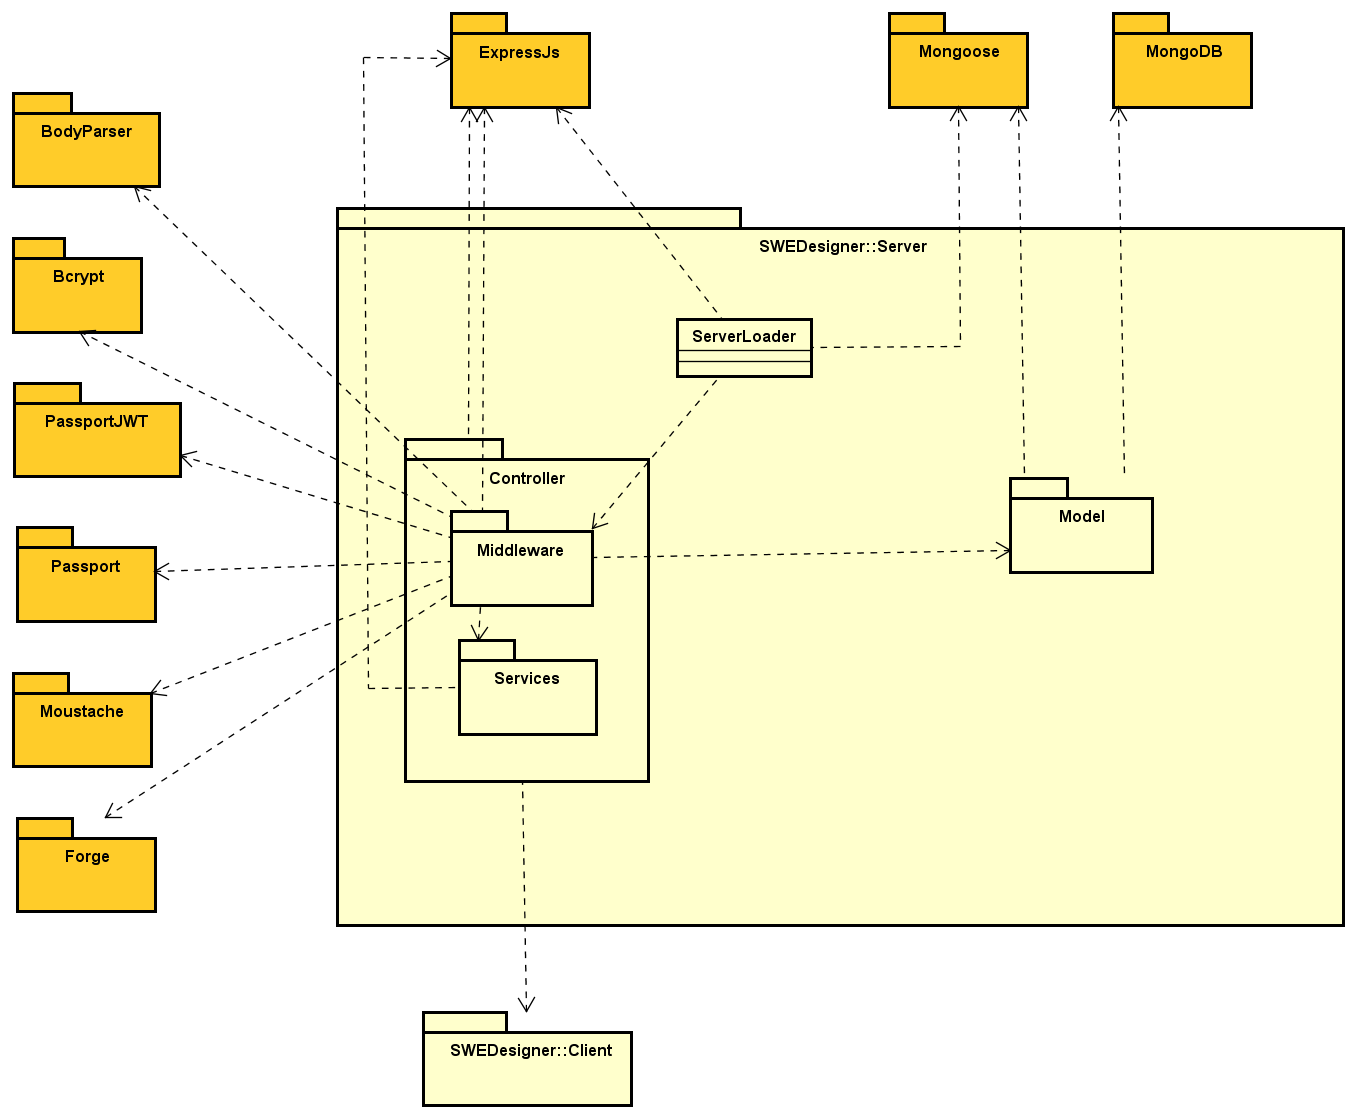
\includegraphics[scale=0.4]{Disegnetti/Back-End.png}
		\caption{Diagramma dei packages SWEDesigner::Server}
 		\end{figure}
		\paragraph{Informazioni sul Package}
		\begin{itemize}
			\item \textbf{Descrizione: }\\
			Package che racchiude tutta la componente del server scritta in JavaScript.
			\item \textbf{Padre: }\\ SWEDesigner
			\item \textbf{Package contenuti: }
			\begin{itemize}
				\item SWEDesigner::Server::Controller;\\
				Questo package contiente tutte le componenti middleware e i servizi con i quali si interfacciano.
				Ogni controller si occupa di gestire tutte le richieste del client attraverso i sui componenti middleware e di rispondere ad esse attraverso
				l'interfaccia REST definita da express.
				\item SWEDesigner::Server::Model;\\
				Questo package contene le classi e i metodi che si interfacciano con il database passando dal modulo di moongose.
				Il model si occupa quindi delle richieste al database e delle operazioni ad esso dedicate rispondendo alle varie richieste del controller.
			\end{itemize}
		\end{itemize}

		\paragraph{Informazioni sulle Classi}
		\begin{itemize}
			\item SWEDesigner::Server::ServerLoader
			\begin{itemize}
				\item \textbf{Descrizione: }\\
				Classe che consente il caricamento del server.
				\item \textbf{Utilizzo: }\\
				La classe viene utilizzata per caricare tutte le componenti del server nel momento dell'avvio dell'applicazione.
			\end{itemize}
		\end{itemize}

		\subsubsection{SWEDesigner::Server::Controller}
		 \begin{figure}[h!]
		\centering
		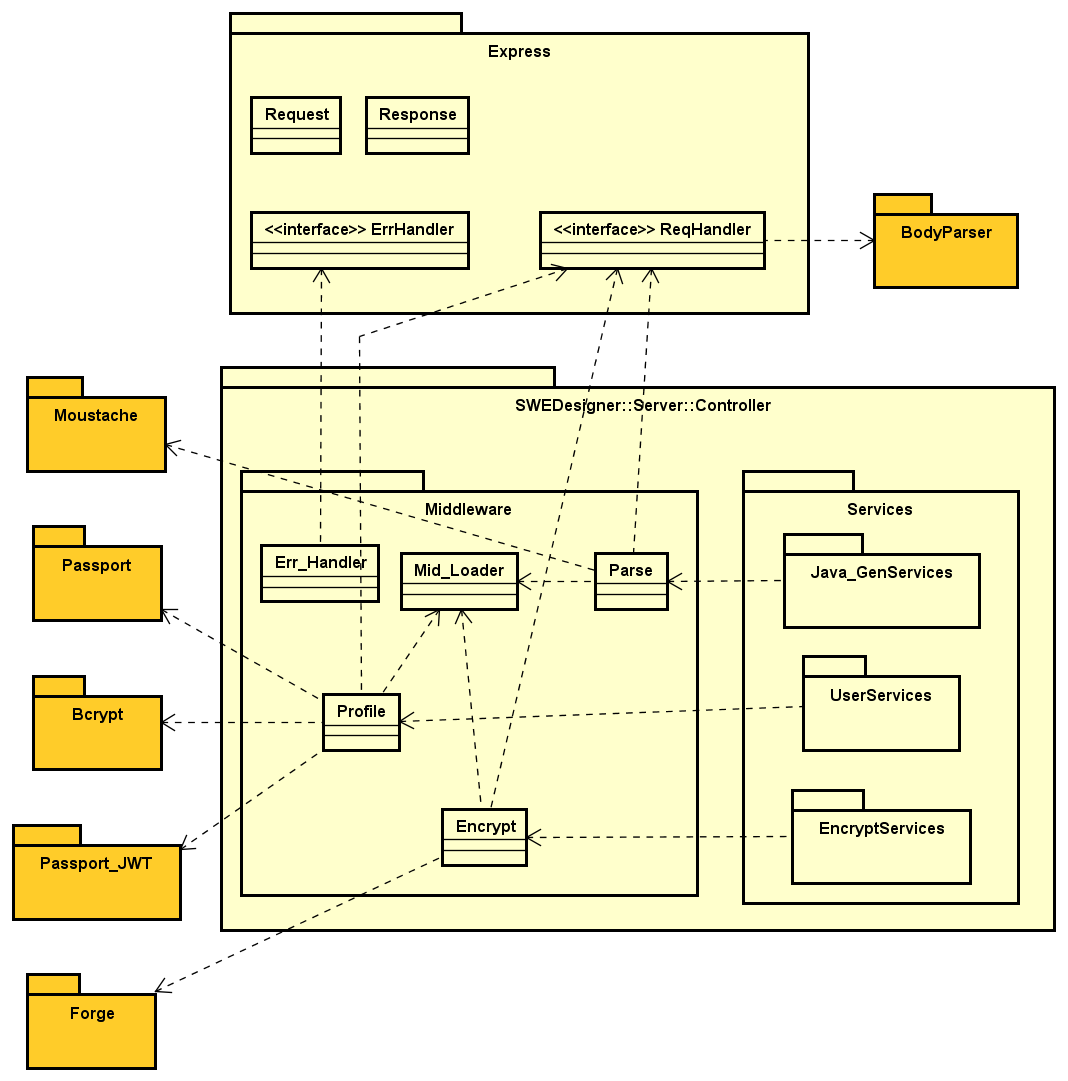
\includegraphics[scale=0.4]{Disegnetti/SWEDesigner__Server__Controller.png}
		\caption{Diagramma dei packages SWEDesigner::Server::Controller}
 		\end{figure}
		\paragraph{Informazioni sul Package}
		\begin{itemize}
			\item \textbf{Descrizione: }\\
			Il package racchiude al suo interno tutti i servizi e le componenti middleware che regolano la bussiness logic del server.
			\item \textbf{Padre: }\\ SWEDesigner::Server
			\item \textbf{Package contenuti: }
			\begin{itemize}
				\item \emph{SWEDesigner::Server::Controller::Middleware};\\
				Si tratta del package contenente tutte le componenti middleware che rispondono alle varie richieste del client.
				\item \emph{SWEDesigner::Server::Controller::Services};\\
				Si tratta del package contentente tutti i servizi utilizzati dalle componenti middleware per il corretto svolgersi delle loro operazioni.
			\end{itemize}
		\end{itemize}

		\subsubsection{SWEDesigner::Server::Controller::Middleware}
		\paragraph{Informazioni sul Package}
		\begin{itemize}
			\item \textbf{Descrizione: }\\
			Si tratta del package contenente tutte le componenti middleware che rispondono alle varie richieste del client.
			\item \textbf{Padre: }\\ SWEDesigner::Server::Controller
		\end{itemize}
		\paragraph{Informazioni sulle Classi}
		\begin{itemize}
			\item SWEDesigner::Server::Controller::Middleware::ErrHandler
			\begin{itemize}
				\item \textbf{Descrizione: }\\
				Si tratta della classe che si occupa della gestione degli errori nelle richieste REST che derivano dal client.
				\item \textbf{Utilizzo: }\\
				La classe, interfacciandosi con un'interfaccia di express, si occupa di gestire, grazie ad una relazione con la realita interfaccia di express, tutti gli errori delle richieste arrivate dal client.
				\item \textbf{Relazioni con le altre classi: }
				\begin{itemize}
					\item \emph{IN} express::ErrHandler
				\end{itemize}
			\end{itemize}
			\item SWEDesigner::Server::Controller::Middleware::MidLoader
			\begin{itemize}
				\item \textbf{Descrizione: }\\
				Si tratta della classe che si occupa di caricare tutte le componenti middleware del server.
				\item \textbf{Utilizzo: }\\
				La classe carica tutte le componenti middelware del servr applicando il design patter \glossaryItem{Facade}.
			\end{itemize}
			\item SWEDesigner::Server::Controller::Middleware::Parse
			\begin{itemize}
				\item \textbf{Descrizione: }\\
				Classe per la gestione del parsing dei file JSON.
				\item \textbf{Utilizzo: }\\
				La classe, utilizzando la componente esterna Moustache, si occupa di fare il parsing dei file JSON in arrivo dal client e creare, tramite il servizio JavaGen, il codice
				sorgente.
				\item \textbf{Relazioni con le altre classi: }
				\begin{itemize}
					\item \emph{IN} MidLoader
					\item \emph{IN} express::ReqHandler
				\end{itemize}
			\end{itemize}
			\item SWEDesigner::Server::Controller::Middleware::Profile
			\begin{itemize}
				\item \textbf{Descrizione: }\\
				Classe per la gestione dei servizi middleware riguardanti l'utente, come registrazione e autenticazione.
				\item \textbf{Utilizzo: }\\
				Con l'ausilio di moduli esterni di Passport	e Bcrypt, la classe si occupa di gestire tutti quei servizi middleware che riguardano il profilo dell'utente.
				\item \textbf{Relazioni con le altre classi: }
				\begin{itemize}
					\item \emph{IN} MidLoader
					\item \emph{IN} express::ReqHandler
				\end{itemize}
			\end{itemize}
			\item SWEDesigner::Server::Controller::Middleware::Encrypt
			\begin{itemize}
				\item \textbf{Descrizione: }\\
				Classe per l'encrypt e il decrypt dei file di progetto.
				\item \textbf{Utilizzo: }\\
				La classe, utilizzando il modulo esterno Forge, encrypta i file di progetto generati tramite SWEDesigner e ne effettua la decrittazione al momento del caricamento
				degli stessi.
				\item \textbf{Relazioni con le altre classi: }
				\begin{itemize}
					\item \emph{IN} MidLoader
					\item \emph{IN} express::ReqHandler
				\end{itemize}
			\end{itemize}
		\end{itemize}


		\subsubsection{SWEDesigner::Server::Controller::Services}
		\paragraph{Informazioni sul Package}
		\begin{itemize}
			\item \textbf{Descrizione: }\\
			Qualcosa
			\item \textbf{Padre: }\\ SWEDesigner::Server::Controller
			\item \textbf{Package contenuti: }
			\begin{itemize}
				\item \emph{SWEDesigner::Server::Controller::Services::JavaGenServices};\\
				Tramite questo package si effettuano tutti i servizi dediti alla generaizone di codice sorgente a partire dagli UML creati dall'utente
				all'intero di SWEDesigner.
				\item \emph{SWEDesigner::Server::Controller::Services::UserServices}
				Il package presenta tutti quei servizi utili alle componenti middleware per la gestione del profilo dell'utente.
			\end{itemize}
		\end{itemize}
		\paragraph{Informazioni sulle Classi}
		\begin{itemize}
			\item SWEDesigner::Server::Controller::Services::EncryptServices
			\begin{itemize}
				\item \textbf{Descrizione: }\\
				La classe offre il servizio di encrypt e decrypt utile alla componente Middleware::Encrypt.
				\item \textbf{Utilizzo: }\\
				Il servizio in questione offre tutti i metodoti utili al middleware per effettuare la criptazione e decrittazione dei file di progetto caricati e salvati dagli utenti.
			\end{itemize}
		\end{itemize}

		\subsubsection{SWEDesigner::Server::Controller::Services::JavaGenService}
		\begin{figure}[h!]
		\centering
		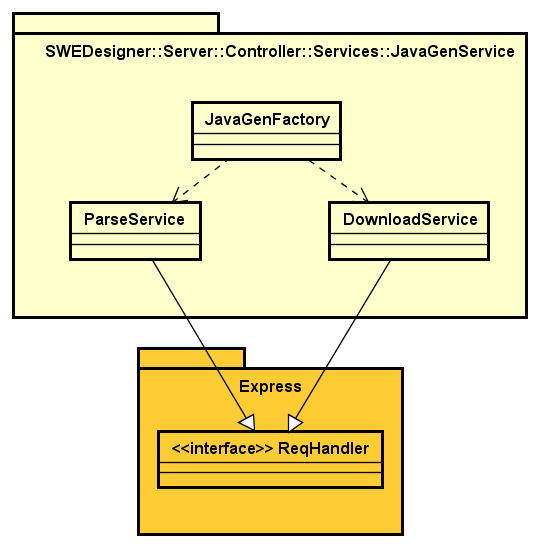
\includegraphics[scale=0.4]{Disegnetti/SWEDesigner__Server__Controller__Services__JavaGenService.png}
		\caption{Diagramma dei packages SWEDesigner::Server::Controller::Services::JavaGenService}
 		\end{figure}
		\paragraph{Informazioni sul Package}
		\begin{itemize}
			\item \textbf{Descrizione: }\\
			Il pacchetto contiente tutti i servizi di generazione e download del codice sorgente a parite dagli UML	disegnati dall'utente.
			\item \textbf{Padre: }\\ SWEDesigner::Server::Controller::Services
		\end{itemize}
		\paragraph{Informazioni sulle Classi}
		\begin{itemize}
			\item SWEDesigner::Server::Controller::Services::JavaGenService::JavaGenFactory
			\begin{itemize}
				\item \textbf{Descrizione: }\\
				La classe implementa il pattern \glossaryItem{Factory} per la creazione di un controller che si occupi di gestire i servizi di generazione codice.
				\item \textbf{Utilizzo: }\\
				La classe viene utilizzata come creator per la creazione del controller dei servizi di generazione, tramite parsing, e download del codice sorgente.
			\end{itemize}
			\item SWEDesigner::Server::Controller::Services::JavaGenService::ParseService
			\begin{itemize}
				\item \textbf{Descrizione: }\\
				La classe effettua il parsing del JSON generato dai diagrammi UML e lo trasforma in codice sorgente Java.
				\item \textbf{Utilizzo: }\\
				Mediante l'utilizzo del modulo esterno Moustache, il servizio si occupa di effettuare il parsing del JSON inviato tramite richista REST dal client e di generare
				il codice sorgente associato.
				\item \textbf{Relazioni con le altre classi: }
				\begin{itemize}
					\item \emph{OUT} Express::ReqHandler
				\end{itemize}
			\end{itemize}
			\item SWEDesigner::Server::Controller::Services::JavaGenService::DownloadService
			\begin{itemize}
				\item \textbf{Descrizione: }\\
				La classe effettua il download del codice sorgente generato a partire dagli UML dell'utente.
				\item \textbf{Utilizzo: }\\
				La classe invia al client che lo ha richiesto lo stream del file .jar sorgente creato a partire dal JSON inviato tramite richiesta REST.
				\item \textbf{Relazioni con le altre classi: }
				\begin{itemize}
					\item \emph{OUT} Express::ReqHandler
				\end{itemize}
			\end{itemize}
		\end{itemize}

		\subsubsection{SWEDesigner::Server::Controller::Services::UserServices}
		\begin{figure}[h!]
		\centering
		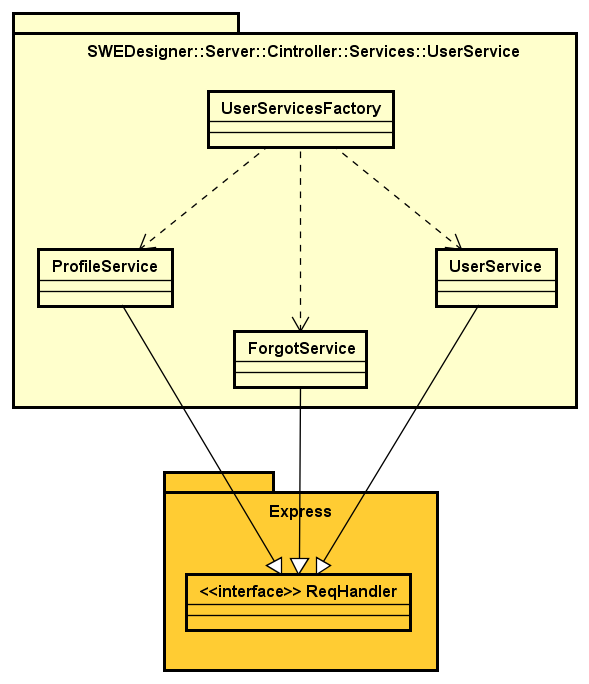
\includegraphics[scale=0.4]{Disegnetti/SWEDesigner__Server__Controller__Services__UserService.png}
		\caption{Diagramma dei packages SWEDesigner::Server::Controller::Services::UserServices}
 		\end{figure}
		\paragraph{Informazioni sul Package}
		\begin{itemize}
			\item \textbf{Descrizione: }\\
			Il packege contiene al suo interno tutti i servizi utili all'utente per l'autenticazione e la gestione del profilo.
			\item \textbf{Padre: }\\ SWEDesigner::Server::Controller::Services

		\end{itemize}
		\paragraph{Informazioni sulle Classi}
		\begin{itemize}
			\item SWEDesigner::Server::Controller::Services::UserServices::UserServicesFactory
			\begin{itemize}
				\item \textbf{Descrizione: }\\
				La classe implementa il patter \glossaryItem{Factory} per la creazione di un controller che gestisca i servizi relativi all'autenticazione e registrazione di un utente.
				\item \textbf{Utilizzo: }\\
				La classe viene utilizzata come creator per la creazione del controller che si occupa dei servizi riguardanti il profilo dell'utente e le sue credenziali.
			\end{itemize}
			\item SWEDesigner::Server::Controller::Services::UserServices::ProfileService
			\begin{itemize}
				\item \textbf{Descrizione: }\\
				La classe gestisce i servizi di autenticazione e registrazione.
				\item \textbf{Utilizzo: }\\
				La classe contiene tutti metodi necessari per l'autenticazione e la registrazione di un utente all'interno del database.
				\item \textbf{Relazioni con le altre classi: }
				\begin{itemize}
					\item \emph{OUT} Express::ReqHandler
				\end{itemize}
			\end{itemize}
			\item SWEDesigner::Server::Controller::Services::UserServices::ForgotService
			\begin{itemize}
				\item \textbf{Descrizione: }\\
				La classe offre il servizio di recupero password.
				\item \textbf{Utilizzo: }\\
				La classe permette all'utente di recuperare le credenziali del proprio account.
				\item \textbf{Relazioni con le altre classi: }
				\begin{itemize}
					\item \emph{OUT} Express::ReqHandler
				\end{itemize}
			\end{itemize}
			\item SWEDesigner::Server::Controller::Services::UserServices::UserService
			\begin{itemize}
				\item \textbf{Descrizione: }\\
				La classe gestisce il profilo dell'utente.
				\item \textbf{Utilizzo: }\\
				La classe offre i servizi di management di un account.
				\item \textbf{Relazioni con le altre classi: }
				\begin{itemize}
					\item \emph{OUT} Express::ReqHandler
				\end{itemize}
			\end{itemize}
		\end{itemize}

		\subsubsection{SWEDesigner::Server::Model}
		 \begin{figure}[h!]
		\centering
		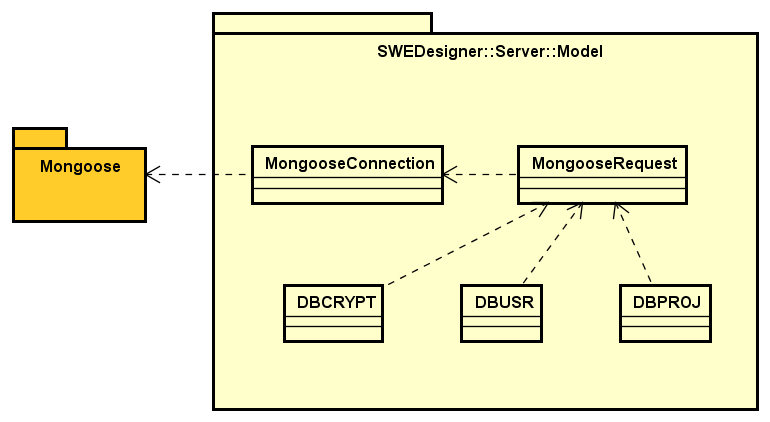
\includegraphics[scale=0.4]{Disegnetti/SWEDesigner__Server__Model.png}
		\caption{Diagramma dei packages SWEDesigner::Server::Model}
 		\end{figure}
		\paragraph{Informazioni sul Package}
		\begin{itemize}
			\item \textbf{Descrizione: }\\
			Il package si occupa delle comunicazioni con il database passando peril modulo di Mongoose per le richieste allo stesso.
			\item \textbf{Padre: }\\ SWEDesigner
		\end{itemize}

		\paragraph{Informazioni sulle Classi}
		\begin{itemize}
			\item SWEDesigner::Server::Model::MongooseConnection
			\begin{itemize}
				\item \textbf{Descrizione: }\\
				La classe stablisce la connessione al database.
				\item \textbf{Utilizzo: }\\
				La classe si connette al database passando per il modulo di Mongoose.
			\end{itemize}
			\item SWEDesigner::Server::Model::Model
			\begin{itemize}
				\item \textbf{Descrizione: }\\
				La classe implementa il pattern \glossaryItem{Facade} per la realizzazione del data tier.
				\item \textbf{Utilizzo: }\\
				La classe fornisce un'interfaccia per le classi che gestiscono il database.
			\end{itemize}
			\item SWEDesigner::Server::Model::DBUSR
			\begin{itemize}
				\item \textbf{Descrizione: }\\
				La classe gestisce il database utenti.
				\item \textbf{Utilizzo: }\\
				La classe fornisce tutti gli strumenti per la lettura e la scrittura di un utente.
			\end{itemize}
			\item SWEDesigner::Server::Model::DBPROJ
			\begin{itemize}
				\item \textbf{Descrizione: }\\
				La classe gestisce il database dei progetti.
				\item \textbf{Utilizzo: }\\
				La classe fornisce tutti gli strumenti per la lettura e la scrittura di un progetto.
			\end{itemize}
		\end{itemize}
